\documentclass[article]{ajs}

\usepackage{booktabs}
\usepackage{amsmath}
\usepackage{amssymb}
\usepackage{xurl}

\author{Tatsuki Onishi\\ Shiga University\\ Data Science AI Innovation
        Research Promotion Center}

\title{IONE: Identifiability-Oriented Navigation of Evidence for Auditing
Aggregate Clinical Trial Data}

\Plainauthor{Tatsuki Onishi}
\Plaintitle{IONE: Identifiability-Oriented Navigation of Evidence for
Auditing Aggregate Clinical Trial Data}
\Shorttitle{IONE: Auditing Aggregate Trial Data}

\Abstract{
Even a well-conducted randomized trial or meta-analysis publishes, at
best, arm-level margins and a few subgroup tables; whether those
aggregates can justify a treatment decision for a particular patient
subgroup is a question of identification, not estimation. We present
\texttt{ione} (IONE: Identifiability-Oriented Navigation of Evidence), an
open-source \proglang{Python} package that audits published aggregate
randomized-trial data without requiring individual patient data. For a
binary stratum, binary outcome, and two-arm design, the set of
conditional risk distributions compatible with the published margins is
a polytope, and \texttt{ione} computes sharp bounds on the stratum-specific
risk difference by linear programming (HiGHS), returning one of five
explicitly disjoint verdicts --- \code{ROBUST\_TREAT},
\code{ROBUST\_NO\_TREAT}, \code{REVERSIBLE}, \code{INFEASIBLE}, or
\code{UNSUPPORTED} --- so that contradictory inputs, missing
specification, and genuine nonidentification are never conflated. When a
decision is not robust, the package orders additional \emph{reportable}
aggregate summaries by burden (re-tabulation before new measurement
before new enrollment) without promising resolution. Audits are organized
as an explicit information ladder: arm-level totals only (L1), plus
stratum denominators (L2), plus arm-by-stratum event counts (L3), so
that a reader can see exactly which published table changes the answer.
Applications to published data show the ladder working in both
directions: in RECOVERY (dexamethasone in hospitalized COVID-19
patients) the published arm-by-stratum counts reach L3 and
point-identify the crude stratum risk differences --- including the
unfavourable direction in the no-oxygen subgroup that lower information
levels leave undecided --- while in ISIS-2 (aspirin and streptokinase in
acute myocardial infarction) subgroup effects were published as odds
reductions but not as arm-by-stratum counts, so the event-count ladder
stops at L1 and names the missing table concretely. A retrospective leave-one-subgroup-out check on RECOVERY
further reproduces a realistic direction reversal that unexamined
pooling would have produced. The tool recommends no treatment; it
reports what each level of published counts identifies and what
reportable information would narrow the bounds.
}
\Keywords{partial identification, aggregate data, clinical trials,
decision analysis, evidence audit, \proglang{Python}}
\Plainkeywords{partial identification, aggregate data, clinical trials,
decision analysis, evidence audit, Python}

\Pages{1--xx}

\Address{
  Tatsuki Onishi\\
  Shiga University, Data Science AI Innovation Research Promotion
  Center\\
  1-1-1 Banba, Hikone, Shiga 522-8522, Japan\\
  E-mail: \email{bougtoir@gmail.com}
}

\begin{document}

\section{Introduction}
\label{sec:intro}

Clinicians and evidence-synthesis researchers routinely face a situation
in which a randomized controlled trial (RCT) or meta-analysis is
statistically sound, yet the published report does not settle the
question that matters in front of them: whether a treatment helps the
specific subgroup their patient belongs to. Trials typically report
arm-level event counts for the whole sample and, occasionally, crude
subgroup tables. Whether those aggregates are even consistent with a
unique subgroup-level treatment effect --- and, if not, how wide the
range of compatible effects is --- is a question of identification, not
of estimation precision.

That published margins do not uniquely determine conditional quantities
is a classical result. Manski's framework of partial identification
\citep{manski2003} formalizes bounds on quantities that remain set-valued
given the available information; \citet{cross2002} showed that aggregate
("short") regressions identify conditional means only up to intervals;
\citet{king1997} obtained deterministic bounds on individual-level
cell probabilities from aggregate two-by-two margins in the ecological
inference literature; and \citet{horowitz2000} derived bounds on
treatment effects in randomized experiments with missing covariate and
outcome data. Linear programming formulations for sharp treatment-effect
bounds under structural assumptions go back to \citet{balke1997}. More
recently, \citet{moon2026} independently developed sharp bounds for
linear combinations of conditional mean outcomes when only group-level
marginal distributions are observed --- mathematically the same family of
marginal-consistency programs that we use, motivated by economic
outcomes. None of this work, however, addresses the applied question a
clinical researcher faces at the level of a published report: given
\emph{this} trial's printed tables, is a decision for \emph{this}
subgroup already determined, could it still reverse, and which
additional \emph{reportable} summary --- one the original investigators
could plausibly supply --- would narrow the answer?

Existing software does not close this gap. Meta-analytic packages
\citep{viechtbauer2010} synthesize published effects but assume the
estimates are already identified. Sensitivity-analysis tools such as the
E-value \citep{vanderweele2017} quantify robustness to unmeasured
confounding for a point-identified estimate --- a different question from
nonidentification. Bound software exists in econometrics --- the
\texttt{tebounds} command \citep{mccarthy2015} and the
\texttt{bpbounds} implementation of the Balke--Pearl bounds
\citep{palmer2011} --- but these require microdata or instrumental-variable
designs and do not operate on published arm-level margins. Transportability
theory \citep{pearlbareinboim2014} identifies conditions under which a
causal effect may be carried to a new population, but presumes assumptions
that a published report rarely documents.

We present \texttt{ione} (IONE: Identifiability-Oriented Navigation of
Evidence), an open-source \proglang{Python} package that turns this
identification question into a reproducible audit. Its contributions are
deliberately those of an applied tool, not of new theory: (i) a complete
audit workflow on published aggregate counts --- consistency checking of
subgroup tables against the overall margin, sharp conditional
risk-difference bounds by linear programming, an explicit L1/L2/L3
information-level ladder that separates deliberate ablations from
genuine publication gaps, and a five-state verdict
taxonomy that keeps inconsistency (\code{INFEASIBLE}), underspecification
(\code{UNSUPPORTED}), and nonidentification (\code{REVERSIBLE}) strictly
separate; (ii) cost-ordered suggestions of additional \emph{reportable}
summaries (re-tabulation of already-collected data before new measurement
before new enrollment), each with its assumptions stated and none
promising resolution; and (iii) two source-verified applications to
landmark trials plus one deliberately excluded counterexample,
including a documented real-data direction reversal that unexamined
subgroup pooling would have produced.
The name IONE also denotes an earlier observational-stratification
framework by the same author (here: ``original/legacy IONE''); the two
share only the name and are distinguished throughout.

The tool does not recommend treatment for any patient, does not claim
external validity, and returns abstention (\code{UNSUPPORTED}) as a
first-class output when the information class is not supported. The
remainder of the paper defines the audit problem and the exact
computation (Section~\ref{sec:methods}), describes the implementation and
its verification (Section~\ref{sec:impl}), reports the real-data audits
(Section~\ref{sec:results}), and discusses scope, limitations, and
relation to prior work (Section~\ref{sec:discussion}).

\section{The audit problem and exact computation}
\label{sec:methods}

\subsection{Data and estimand}

We consider the smallest setting in which the problem already bites: a
binary stratum indicator $X \in \{0,1\}$ (e.g., ``receiving no
respiratory support at randomization''), a binary outcome $Y \in \{0,1\}$
(e.g., death within 28 days), and two arms $T \in \{0,1\}$ (control,
treatment). The published report supplies arm-level margins
$\bar p_0 = P(Y{=}1 \mid T{=}0)$ and $\bar p_1 = P(Y{=}1 \mid T{=}1)$ ---
overall event risks per arm --- and a subgroup table that supplies, for
each named stratum, the arm-specific counts $(e_{1x}, n_{1x})$ and
$(e_{0x}, n_{0x})$, from which the stratum prevalence $q = P(X{=}1)$ (or
arm-specific prevalences $q_0, q_1$) is estimated. The estimand is the
stratum-specific risk difference
\[
\mathrm{RD}_x \;=\; P(Y{=}1 \mid T{=}1, X{=}x) - P(Y{=}1 \mid T{=}0, X{=}x),
\qquad x \in \{0,1\}.
\]

Write the four latent conditional risks as
$\theta = (p_{00}, p_{01}, p_{10}, p_{11})$ where $p_{tx} = P(Y{=}1 \mid
T{=}t, X{=}x)$. The published margins impose the linear equalities
\begin{equation}
(1-q)\, p_{0,0} + q\, p_{0,1} = \bar p_0, \qquad
(1-q)\, p_{1,0} + q\, p_{1,1} = \bar p_1,
\label{eq:margins}
\end{equation}
and $\theta \in [0,1]^4$. If the report additionally publishes a
per-stratum outcome margin $P(Y{=}1 \mid X{=}x)$, the constraint
$(1 - m_x)\, p_{0x} + m_x\, p_{1x} = P(Y{=}1 \mid X{=}x)$ applies, where
$m_x = P(T{=}1 \mid X{=}x)$ must be supplied by the analyst --- it is
never defaulted to the allocation ratio. Because all constraints are
linear and the feasible set $\Theta$ is a polytope, the sharp bounds of
the linear estimand $\mathrm{RD}_x = p_{1x} - p_{0x}$ are obtained
exactly by two linear programs,
\[
\mathrm{RD}_x^{-} = \min_{\theta \in \Theta} (p_{1x} - p_{0x}), \qquad
\mathrm{RD}_x^{+} = \max_{\theta \in \Theta} (p_{1x} - p_{0x}),
\]
solved with the HiGHS dual simplex solver
\citep{huangfu2018, scipy2020}. ``Sharp'' is used in the standard
sense: the interval is the tightest one implied by \eqref{eq:margins}
alone; both endpoints are attained by feasible conditional
distributions.

Three conditions govern interpretation. First, the bounds are
\emph{identification bounds on the published margins}, not confidence
intervals: sampling uncertainty in the reported counts is a separate
layer that we do not model here \citep[cf.][]{imbens2004}. Second, when
arm compositions differ ($q_1 \neq q_0$), each arm uses its own stratum
prevalence; a single common $q$ is used only when the arm shares are
compatible. At L2 the prevalences themselves come from the published
denominators and are likewise conditioned on as given, not treated as
exact population quantities. Third, nothing in \eqref{eq:margins} restricts
unmeasured-effect-modifier structures beyond $X$; declaring a suspected
unmeasured modifier changes only the augmentation advice
(Section~\ref{sec:aug}), not the bounds.

\subsection{Verdicts}

Given a decision threshold $\tau \ge 0$ on the adverse-event scale
(benefit requires $\mathrm{RD}_x < -\tau$), the audit returns exactly one
of five disjoint states:

\begin{itemize}
\item \code{ROBUST\_TREAT}: every model in $\Theta$ gives
      $\mathrm{RD}_x < -\tau$;
\item \code{ROBUST\_NO\_TREAT}: every model in $\Theta$ gives
      $\mathrm{RD}_x > -\tau$;
\item \code{REVERSIBLE}: $\Theta$ contains models on both sides of
      $-\tau$ (genuine nonidentification of the decision);
\item \code{INFEASIBLE}: $\Theta$ is empty --- the published aggregates
      are mutually inconsistent;
\item \code{UNSUPPORTED}: the input lacks a required specification
      (stratum prevalence, arm mixing proportion) or the solver fails.
\end{itemize}

These are the five \emph{primary} states. For backward compatibility
the implementation retains two legacy aliases, \code{SUFFICIENT} and
\code{UNIDENTIFIABLE}, from the original IONE vocabulary; they are
distinct enum values kept only so older callers do not break, and the
audit outputs here never emit them.

The \code{ROBUST} labels refer exclusively to sign stability within
the identified set conditional on the observed margins and stated
assumptions; they do not incorporate sampling uncertainty and do not
constitute clinical treatment recommendations.

The separation matters in practice: \code{INFEASIBLE} points to a
reporting error worth querying, \code{UNSUPPORTED} to missing analyst
input, and \code{REVERSIBLE} to an information gap in the literature
--- three different actions.

\subsection{Information levels}
\label{sec:levels}

Because the audit's purpose is to show \emph{which} published table
carries the answer, every stratum audit is reported as a ladder of
three explicitly defined information levels, for one and the same
estimand (the stratum-specific crude risk difference):

\begin{itemize}
\item \textbf{L1} (arm totals only): overall arm-level event counts;
      stratum denominators and events withheld. The stratum risk
      difference is unidentified with the trivial identified set
      $[-1, +1]$.
\item \textbf{L2} (plus stratum denominators): the arm-by-stratum
      sample sizes (equivalently the stratum prevalences $q_0, q_1$)
      are added, imposing \eqref{eq:margins}; the sharp LP bounds
      apply.
\item \textbf{L3} (plus stratum event counts): the arm-by-stratum
      outcome counts are added. Two independent equations collapse
      $\Theta$ to a point: the crude stratum risk difference is
      point-identified and equals the difference of the published
      proportions. A confidence interval around that point is
      \emph{sampling} uncertainty and is reported separately --- it
      is never mixed into the identified set.
\end{itemize}

Two interpretive rules are fixed. First, L1 and L2 are
\emph{deliberate ablations} when L3 information was actually
published: they measure what a reader who ignored the arm-by-stratum
table could still conclude, and must never be described as a genuine
publication gap. A level is called a gap only when the information
was never reported (as in the ISIS-2 example below). Second,
point-identification at L3 is identification of an \emph{aggregate
stratum contrast}, not of any individual's causal effect: its causal
reading requires randomization, a pre-treatment stratum definition,
complete outcome ascertainment, and the usual estimand conditions,
all of which are stated rather than assumed away.

\subsection{Consistency checking}
\label{sec:consistency}

Before the LP is run, subgroup counts are checked against the overall
table: for exhaustive strata, sums of events and denominators must equal
the overall counts; small gaps are flagged as warnings (rounding or an
unpublished stratum), while exceedances are errors that render the audit
\code{INFEASIBLE}. Duplicate stratum names are treated as overlap errors.
This check is cheap and frequently pays: subgroup tables that cannot
support any conclusion are identified before any bounds are computed.

\subsection{Reportable augmentation}
\label{sec:aug}

When the verdict is \code{REVERSIBLE} or \code{UNSUPPORTED}, the package
lists additional aggregate summaries the original investigators could in
principle supply, ordered by expected burden:

\begin{enumerate}
\item \emph{re-tabulation} (near-zero cost): an arm $\times$ stratum
      outcome cross-tabulation, or per-stratum baseline risk;
\item \emph{new measurement} on existing cohorts;
\item \emph{new enrollment}: a stratum-restricted randomized cohort;
\item \emph{abstain}: no publishable summary is shown to resolve the
      decision.
\end{enumerate}

For the binary-stratum model, an arm $\times$ stratum cross-tabulation
adds two independent equations and collapses $\Theta$ to a point ---
identifiability is structural. Every option is classified
(\texttt{sufficient\_assumed}, \texttt{potentially\_informative},
\texttt{irrelevant}, \texttt{infeasible}, \texttt{unknown}) together with
the assumptions under which its classification holds; no option carries
an unconditional guarantee of resolution, since the future cells are
unknown a priori.

\subsection{Retrospective borrow check}

As a demonstration diagnostic --- not a borrowing method --- the package
pools the other subgroups' log risk ratios (fixed effect) and compares
the prediction with the held-out subgroup's actual crude risk ratio. The
comparison is retrospective by construction: it documents what unexamined
pooling would have concluded on already-published data, not prospective
validation, and it uses crude rather than adjusted effects.

\section{Implementation and verification}
\label{sec:impl}

\begin{sloppypar}
The package \texttt{ione} (distribution name \texttt{ione-audit}, version
0.2.0) is pure \proglang{Python} depending only on NumPy
\citep{numpy2020} and SciPy \citep{scipy2020}, with the LP solved by
HiGHS \citep{huangfu2018}. It provides a Python API with functions
\code{audit\_decision}, \code{audit\_levels},
\code{suggest\_augmentation}, \code{borrow\_check}, and
\code{EffectSummary.check\_consistency}, and a
command-line interface (\code{ione audit}, \code{ione borrow-check})
emitting structured JSON. Source, tests, and documentation are at
\url{https://github.com/bougtoir/ione-stratification-framework}.
\end{sloppypar}

Verification is algebraic rather than self-referential. For the
two-by-two-by-two model the sharp bounds have a closed form: solving
\eqref{eq:margins} for $p_{t,1}$ given free $p_{t,0}$ and intersecting
the resulting windows yields $\mathrm{RD}_1^- = c - k\,d_{\max}$ and
$\mathrm{RD}_1^+ = c - k\,d_{\min}$ with $c = (\bar p_1 - \bar p_0)/q$,
$k = (1-q)/q$, and $d_{\min}, d_{\max}$ the range of $p_{1,0} - p_{0,0}$
over the feasible windows. The test suite checks LP optima against this
closed form (agreement to $10^{-8}$ on curated cases; $1.8 \times
10^{-15}$ worst case over 200 random margins), against coarse full
enumeration (sign agreement), and against published effect estimates
(crude risk ratios for all three datasets, Haldane-corrected odds ratios
for zero cells). Edge cases are asserted explicitly: missing prevalence
returns \code{UNSUPPORTED}, inconsistent margins return
\code{INFEASIBLE}, prevalence near 1 collapses bounds to the marginal
risk difference, and prevalence near 0 widens them to $[-1, 1]$. For the
information ladder, a regression test asserts on random margin-consistent
inputs that adding constraints never enlarges the identified set
(L1 $\supseteq$ L2 $\supseteq$ L3 point), and unreachable levels return
\code{UNSUPPORTED}. All 34
tests pass under Python 3.9, 3.11, and 3.12 in continuous integration.

\section{Applications to published trials}
\label{sec:results}

Table~\ref{tab:data} summarizes the three source datasets; all counts
are transcribed from the primary publications and cross-verified (the
RECOVERY counts match the primary report \citep{recovery2021}
percentage-for-percentage; ISIS-2 from \citet{isis2_1988}; REACT from
\citet{react2020}). We report crude estimates only; where the original
study's headline was model-adjusted (RECOVERY's age-adjusted rate
ratios, REACT's fixed-effect odds ratio), that is noted rather than
treated as the same estimand as a crude risk difference.

\begin{table}[t!]
\centering
\caption{\label{tab:data} Source-verified published aggregate datasets
used for the audits (crude arm-level counts): RECOVERY
\citep{recovery2021}, ISIS-2 \citep{isis2_1988}, and WHO REACT
\citep{react2020}.}
\smallskip
{\small
\begin{tabular}{@{}llll@{}}
\toprule
study & outcome & stratum & events/$n$, treat vs.\ control \\
\midrule
RECOVERY & 28-day & overall & 482/2104 vs.\ 1110/4321 \\
(NEJM 2021) & mortality & invasive ventilation & 95/324 vs.\ 283/683 \\
& & oxygen only & 298/1279 vs.\ 682/2604 \\
& & no oxygen & 89/501 vs.\ 145/1034 \\
\midrule
ISIS-2 & 5-week vascular & aspirin contrast & 804/8587 vs.\ 1016/8600 \\
(Lancet 1988) & mortality & streptokinase contrast & 791/8592 vs.\ 1029/8595 \\
& & both vs.\ neither & 343/4292 vs.\ 568/4300 \\
& & time-from-onset strata & odds reductions only$^a$ \\
\midrule
REACT & 28-day & overall & 222/678 vs.\ 425/1025 \\
(JAMA 2020) & mortality & serious adv.\ events$^b$ & 64/354 vs.\ 80/342 \\
\bottomrule
\multicolumn{4}{@{}p{\textwidth}@{}}{\footnotesize $^a$Published only
as odds reductions by time from pain onset (35\% SD 6, 16\% SD 7, 21\%
SD 12 for streptokinase); arm-by-stratum denominators and counts were
never reported.}\\
\multicolumn{4}{@{}p{\textwidth}@{}}{\footnotesize $^b$A post-treatment
outcome, not a pre-treatment stratum --- retained only as a documented
counterexample; see text.}
\end{tabular}
}
\end{table}

Table~\ref{tab:levels} reports the information-level audits at threshold
$\tau = 0$ (all demonstrations use this threshold; audits at other
thresholds require an explicit user-specified analysis, which we do
not separately validate here), and Figure~\ref{fig:levels} shows the
identified sets graphically.

\paragraph{RECOVERY.} RECOVERY publishes all three levels, so the ladder
is a pure ablation experiment: at L1 and L2 (arm totals, plus stratum
denominators) every stratum is \code{REVERSIBLE} --- for the minority
no-oxygen stratum the L2 bounds span essentially $[-1,+1]$ --- while the
arm-by-stratum counts at L3 point-identify the crude risk differences:
$-0.121$ (95\%~CI $-0.183$ to $-0.059$) under invasive ventilation,
$-0.029$ ($-0.058$ to $-0.000$) under oxygen only, and $+0.037$
($-0.002$ to $+0.077$) under no oxygen --- point-identification of the
direction, while the 95\%~CI crossing zero records the separate
sampling-uncertainty layer. The ablation makes the role of
each table explicit: the published subgroup counts are what carry the
stratum conclusions, and the no-oxygen subgroup's unfavourable direction
--- which its age-adjusted rate ratio (1.19, a distinct estimand)
reflects --- is invisible at L2.

\paragraph{ISIS-2.} The factorial design's overall contrasts are
published at L3-equivalent completeness (aspirin $-0.024$, streptokinase
$-0.028$, both vs.\ neither $-0.052$ crude risk differences), but for
patient strata --- the report's own time-from-pain-onset subgroups ---
only odds reductions were printed, without arm-by-stratum denominators
or event counts. The ladder for those strata therefore stops at L1 ---
a property of the event-count ladder, not an absence of published
subgroup evidence: the report does contain stratified effect summaries,
just not in the count form that the audit requires. L2 and L3 are
genuinely unreachable, and the augmentation request is
concrete --- the arm $\times$ onset-time outcome cross-tabulation that
was analyzed but not reported. We do not invent the missing table.

\paragraph{REACT.} The REACT serious-adverse-events counts are retained
only as a counterexample: a serious adverse event is a post-treatment
outcome, not a pre-treatment patient characteristic, so it cannot define
a stratum and is excluded from the applications. Screening whether a
candidate variable is a pre-treatment stratum is part of the audit's
input contract, not a numeric check --- this is precisely the kind of
table misuse it exists to block.

\begin{table}[t!]
\centering
\caption{\label{tab:levels} Information-level audits on published data
(threshold $\tau = 0$). Identified sets are reported per level; at L3
the set is a point (crude risk difference) and the bracketed interval is
the 95\%~CI, which is sampling uncertainty, not an identification bound.
L1/L2 are deliberate ablations where L3 was published (RECOVERY); for
ISIS-2 patient strata, L2/L3 are genuinely unreachable because only odds
reductions were published.}
\smallskip
{\small
\begin{tabular}{@{}llll@{}}
\toprule
study: stratum & L1 & L2 & L3 \\
\midrule
RECOVERY: invasive vent.\ & $[-1.00,+1.00]$ & $[-1.00,+1.00]$ &
$-0.121$ [$-0.183,-0.059$] \\
RECOVERY: oxygen only & $[-1.00,+1.00]$ & $[-0.43,+0.38]$ &
$-0.029$ [$-0.058,-0.000$] \\
RECOVERY: no oxygen & $[-1.00,+1.00]$ & $[-1.00,+0.96]$ &
$+0.037$ [$-0.002,+0.077$] \\
ISIS-2: onset-time stratum & $[-1.00,+1.00]$ & --- & --- \\
\bottomrule
\end{tabular}
}
\end{table}

\begin{figure}[t!]
\centering
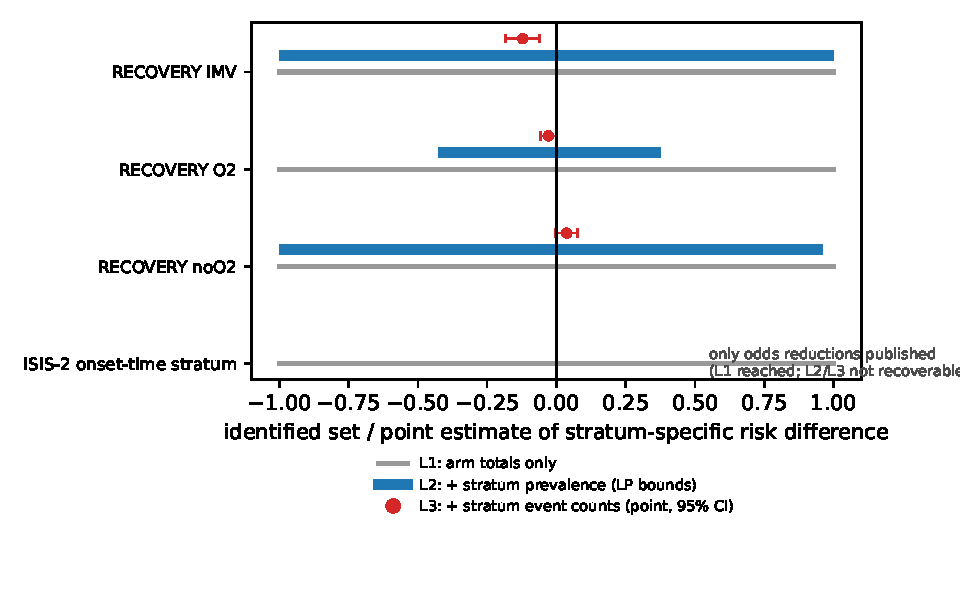
\includegraphics[width=0.8\textwidth]{fig_levels.pdf}
\caption{\label{fig:levels} Identified sets by information level. Grey:
L1 (arm totals only); blue: L2 (plus stratum denominators, LP bounds);
red point and whiskers: L3 (plus arm-by-stratum counts; point with
95\%~CI). For ISIS-2 patient strata only L1 is reachable. For RECOVERY,
L1/L2 are ablations of genuinely published L3 tables.}
\end{figure}

The borrow check illustrates why the audit matters. On RECOVERY, pooling
the other subgroups (invasive ventilation and oxygen only) predicts
benefit for the untreated subgroup --- risk ratio 0.835
(95\%~CI 0.755--0.923) --- while the actual published no-oxygen estimate
shows harm, risk ratio 1.267 (0.995--1.613), with non-overlapping
intervals. This is a retrospective demonstration on real published
counts, not prospective validation of any borrowing rule; it documents
that direction reversal under unexamined pooling is not hypothetical.

For the \code{REVERSIBLE} RECOVERY cases, the augmentation list begins
with a zero-cost option: an arm $\times$ respiratory-support outcome
cross-tabulation of already-collected trial data, which would collapse
the identified interval to a point if produced (the future cell values
remain unknown, so the post-information decision is not guaranteed ---
the classification states this). Per-stratum baseline risk and a
stratum-restricted randomized cohort follow in burden order.

Audits run at interactive speed: each LP pair solves in under a
millisecond, and the full reproduction script (200 random-margin
checks, a 400-point prevalence sweep, all audits and figures) completes
in seconds on a laptop.

\section{Discussion}
\label{sec:discussion}

\subsection{What the audit adds}

The contribution of \texttt{ione} is a reproducible statistical audit
workflow, not a new estimator: partial identification of conditional
quantities from aggregate margins is classical
\citep{cross2002, manski2003, king1997}, the LP formulation follows
\citet{balke1997}, and the same marginal-consistency program has
recently been developed independently for economic outcomes
\citep{moon2026}. What was missing, and what the package supplies, is an
applied layer that a clinical researcher can run on a published report:
consistency screening of the printed tables, sharp bounds with a
decision-verdict taxonomy that separates ``the data contradict
themselves'' from ``the data do not decide'' from ``you have not given
me enough specification,'' and an ordered list of what could still be
reported to narrow the answer --- starting with re-tabulations that cost
the original investigators nothing.

\subsection{Practical uses and the value of abstention}

Three uses appear immediate. First, citation hygiene: a clinician citing
a subgroup result can check which information level the published report
actually reaches --- the RECOVERY ablation shows that dropping the
arm-by-stratum table leaves every stratum decision-reversible, while
ISIS-2 shows a landmark trial whose subgroup reporting never reached
past L1. Second,
requests for re-analysis: the augmentation ordering converts
``we need IPD'' --- usually a dead end --- into a concrete, minimal,
zero-cost request (an arm $\times$ stratum cross-tabulation) that trial
groups can often supply. Third, a disciplined abstention state:
\code{UNSUPPORTED} is an output, not an error, so incomplete reports end
in an explicit statement of what is missing rather than silence.

\subsection{Limitations}

The current release handles binary strata, binary outcomes, and two arms
only; richer covariates enlarge the polytope and are future work. Bounds
are identification bounds on the published margins treated as exact ---
sampling uncertainty in the reported counts is not propagated, and
valid confidence sets for partially identified parameters are a
separate known layer \citep{imbens2004}. Estimands are crude: adjusted
published estimates cannot be reproduced from aggregate counts and are
never substituted for them. The stratum prevalence (or arm-specific
prevalences) must be estimable from the report, which restricts
applicability to trials that publish subgroup denominators --- that
availability is itself the binding real-world constraint. The borrow
check is a retrospective diagnostic, not a validated borrowing method,
and crude risk ratios may differ from adjusted ones. The demonstrations
are drawn from cardiovascular and respiratory trials; the workflow is
domain-agnostic but its value across other specialties is untested.
Finally, the audit audits identifiability, not truth: biased underlying
estimates produce faithful bounds around biased margins.

\subsection{Relation to further work}

The framework complements, rather than competes with, sensitivity
analysis \citep{vanderweele2017} and transportability
\citep{pearlbareinboim2014}: those approaches ask whether conclusions
survive bias or transfer across populations under assumptions, while the
audit asks what the published numbers alone identify under the stated
model. Extensions worth pursuing are interval-valued margins that carry
sampling error, multi-level and continuous strata, and joint audits
across linked trial reports.

\section{Conclusions}
\label{sec:conclusions}

Published aggregate trial data carry more decision-relevant information
than they are usually credited with --- and less than subgroup headlines
suggest. \texttt{ione} makes the gap explicit and reproducible: sharp
identification bounds on subgroup decisions, a verdict taxonomy that
never conflates inconsistency, underspecification, and
nonidentification, and a cost-ordered path to what could still be
reported. The information-level framing makes the examples speak both
ways: RECOVERY shows published arm-by-stratum counts carrying stratum
decisions to L3, while ISIS-2 shows the audit stopping honestly at L1
and naming the missing table. A retrospective borrow check reproduces
a real direction reversal that unexamined pooling would have produced.
The practical value is a disciplined ``we do not know, and here is the
cheapest thing that would tell us'' instead of either over-claiming or
silence.

\bibliography{ione_ajs}

\end{document}
